 \documentclass{article}

\usepackage{fancyhdr}
\usepackage{extramarks}
\usepackage{amsmath}
\usepackage{amsthm}
\usepackage{amsfonts}
\usepackage{amssymb}
\usepackage{xparse}
\usepackage{tikz}
\usepackage{graphicx}
\usepackage[plain]{algorithm}
\usepackage{algpseudocode}
\usepackage{listings}
\usepackage{hyperref}
\usepackage[per-mode = fraction]{siunitx}
\usepackage{calc}
\usepackage{cancel}

\usetikzlibrary{automata,positioning}

\hypersetup{
    colorlinks=true,
    linkcolor=blue,
    filecolor=magenta,
    urlcolor=blue,
    }

\urlstyle{same}

%
% Basic Document Settings
%

\topmargin=-0.45in
\evensidemargin=0in
\oddsidemargin=0in
\textwidth=6.5in
\textheight=9.0in
\headsep=0.25in

\linespread{1.1}

\pagestyle{fancy}
\lhead{\hmwkAuthorName}
\chead{\hmwkClass\ (\hmwkClassInstructor,\ \hmwkClassTime): \hmwkTitle}
\rhead{\firstxmark}
\lfoot{\lastxmark}
\cfoot{\thepage}

\renewcommand\headrulewidth{0.4pt}
\renewcommand\footrulewidth{0.4pt}

\setlength\parindent{0pt}
\allowdisplaybreaks
%
% Title Page
%

\title{
	\vspace{2in}
	\textmd{\textbf{\hmwkClass}}\\
	\textmd{\textbf{\hmwkTitle:}\ \hmwkSubTitle}\\
	\normalsize\vspace{0.1in}\small{Due\ on\ \hmwkDueDate\ at \hmwkDueTime}\\
	\vspace{0.1in}\large{\textit{\hmwkClassInstructor,\ \hmwkClassTime}}
	\vspace{3in}
}
\author{\textbf{\hmwkAuthorName}}
\date{\hmwkCompletionDate}

%
% Create Problem Sections
%

\newcommand{\enterProblemHeader}[1]{
	\nobreak\extramarks{}{Problem #1 continued on next page\ldots}\nobreak{}
	\nobreak\extramarks{Problem #1 (continued)}{Problem #1 continued on next page\ldots}\nobreak{}
}

\newcommand{\exitProblemHeader}[1]{
	\nobreak\extramarks{Problem #1 (continued)}{Problem #1 continued on next page\ldots}\nobreak{}
	\nobreak\extramarks{Problem #1}{}\nobreak{}
}

%
% Homework Problem Environment
%
\NewDocumentEnvironment{hwkProblem}{m m s}{
	\section*{Problem #1: #2}
	\enterProblemHeader{#1}
	\setcounter{partCounter}{1}
}{
	\exitProblemHeader{#1}
	\IfBooleanF{#3} % if star, no new page
		{\newpage}
}

% Alias for the Solution section header
\newcommand{\hwkSol}{\vspace{\baselineskip / 2}\textbf{\Large Solution}\vspace{\baselineskip / 2}}

% Alias for the Solution Part subsection header
\newcounter{partCounter}
\newcommand{\hwkPart}{
	\vspace{\baselineskip / 2}
	\textbf{\large Part \Alph{partCounter}}
	\vspace{\baselineskip / 2}
	\stepcounter{partCounter}
}

%
% Various Helper Commands
%

% Such That
\newcommand{\st}{\text{s.t.}}

% Useful for algorithms
\newcommand{\alg}[1]{\textsc{\bfseries \footnotesize #1}}

% For derivatives
\newcommand{\deriv}[1]{\frac{\mathrm{d}}{\mathrm{d}x} (#1)}

% For partial derivatives
\newcommand{\pderiv}[2]{\frac{\partial}{\partial #1} (#2)}

% Integral dx
\newcommand{\dx}{\mathrm{d}x}
\newcommand{\dy}{\mathrm{d}y}

% Probability commands: Expectation, Variance, Covariance, Bias
\newcommand{\e}[1]{\mathrm{e}#1}
\newcommand{\E}{\mathrm{E}}
\newcommand{\Var}{\mathrm{Var}}
\newcommand{\Cov}{\mathrm{Cov}}
\newcommand{\Bias}{\mathrm{Bias}}

% Col and Row Vectors
\newcommand{\crvector}[1]{\ensuremath{\begin{pmatrix}#1\end{pmatrix}}}

% Defining Units that are not in the SI base
\DeclareSIUnit\bar{bar}
\DeclareSIUnit\ft{ft}
\DeclareSIUnit\dollar{\$}
\DeclareSIUnit\cent{\text{\textcent}}
\DeclareSIUnit\c{\degreeCelsius}

% Code Listing config
\usepackage{xcolor}
\definecolor{codegreen}{rgb}{0,0.6,0}
\definecolor{codegray}{rgb}{0.5,0.5,0.5}
\definecolor{codepurple}{rgb}{0.58,0,0.82}
\definecolor{backcolour}{rgb}{0.95,0.95,0.92}
\lstdefinestyle{overleaf}{
	% backgroundcolor=\color{backcolour},
	commentstyle=\color{codegreen},
	keywordstyle=\color{magenta},
	numberstyle=\tiny\color{codegray},
	stringstyle=\color{codepurple},
	basicstyle=\ttfamily\footnotesize,
	breakatwhitespace=false,
	breaklines=true,
	captionpos=b,
	keepspaces=true,
	numbers=left,
	numbersep=5pt,
	showspaces=false,
	showstringspaces=false,
	showtabs=false,
	tabsize=4
}

% \usepackage[latte]{catppuccinpalette}
% \lstdefinestyle{catppuccin}{
% 	breaklines=true,
% 	keepspaces=true,
% 	numbers=left,
% 	numbersep=5pt,
% 	showspaces=false,
% 	showstringspaces=false,
% 	breakatwhitespace=true,
% 	tabsize=4,
% 	stringstyle = {\color{CtpGreen}},
% 	commentstyle={\color{CtpOverlay1}},
% 	basicstyle = {\small\color{CtpText}\ttfamily},
% 	keywordstyle = {\color{CtpMauve}},
% 	keywordstyle = [2]{\color{CtpBlue}},
% 	keywordstyle = [3]{\color{CtpYellow}},
% 	keywordstyle = [4]{\color{CtpLavender}},
% 	keywordstyle = [5]{\color{CtpPeach}},
% 	keywordstyle = [6]{\color{CtpTeal}}
% }

\lstset{style=overleaf}


%
% Homework Details
%   - Title
%   - Due date
%   - Due time
%   - Course
%   - Section/Time
%   - Instructor
%   - Author
%

\newcommand{\hmwkTitle}{Lab 05}
\newcommand{\hmwkDueDate}{\today}
\newcommand{\hmwkDueTime}{11:59 PM}
\newcommand{\hmwkClass}{ENAE 380}
\newcommand{\hmwkClassTime}{0106}
\newcommand{\hmwkClassInstructor}{Dr. Mumu Xu}
\newcommand{\hmwkAuthorName}{\textbf{Vai Srivastava}}
\newcommand{\hmwkCompletionDate}{\today}

\begin{document}

\maketitle

\pagebreak

\begin{hwkProblem}{3.1.3}{Color Filtering}

	It took my computer 0.05410289764404297 seconds to run the numpy variant, and 0.053965091705322266 seconds to run the python variant.

\end{hwkProblem}

\begin{hwkProblem}{3.4}{Image Segmentation}
		
	Instead of finding a color combination that works for all of the images, I simply created an array with individual highlight and shadow HSV tuples to be used with each image:

	\begin{lstlisting}[language=python]
		# define highlight and shadow ranges for each tiger image
		highlights_hsv = [
		(20, 255, 255),
		(17.5, 255, 255),
		(20, 255, 255),
		(20, 255, 255),
		(45, 255, 255),
		]
		shadows_hsv = [
		(0, 0, 0),
		(10, 0, 0),
		(0, 0, 0),
		(0, 0, 0),
		(0, 0, 0),
		]
	\end{lstlisting}

	\begin{figure}[ht!]
	  \centering
	  \includegraphics[width=0.75\textwidth]{./tigers/3.4.1.png}
	  \caption{Tiger Segmented 1}
	\end{figure}

	\begin{figure}[ht!]
	  \centering
	  \includegraphics[width=0.75\textwidth]{./tigers/3.4.2.png}
	  \caption{Tiger Segmented 2}
	\end{figure}

	\begin{figure}[ht!]
	  \centering
	  \includegraphics[width=0.75\textwidth]{./tigers/3.4.3.png}
	  \caption{Tiger Segmented 3}
	\end{figure}

	\begin{figure}[ht!]
	  \centering
	  \includegraphics[width=0.75\textwidth]{./tigers/3.4.4.png}
	  \caption{Tiger Segmented 4}
	\end{figure}

	\begin{figure}[ht!]
	  \centering
	  \includegraphics[width=0.75\textwidth]{./tigers/3.4.5.png}
	  \caption{Tiger Segmented 5}
	\end{figure}

\end{hwkProblem}

\begin{hwkProblem}{3.5}{Astronomy Image Processing}

	To create these images, I used \lstinline{MAST} to download the \lstinline{FITS} files, then used \lstinline{Siril} to convert the files into a linear colorspace that is viewable for humans, and to register the images such that the stars are all aligned. Then I used \lstinline{Photoshop} to modify the Hue for each image layer and composite them all together.
		
	\begin{figure}[ht!]
	  \centering
	  \includegraphics[width=0.75\textwidth]{./pillars/original.png}
	  \caption{Pillars of Creation Original}
	\end{figure}

	\begin{figure}[ht!]
	  \centering
	  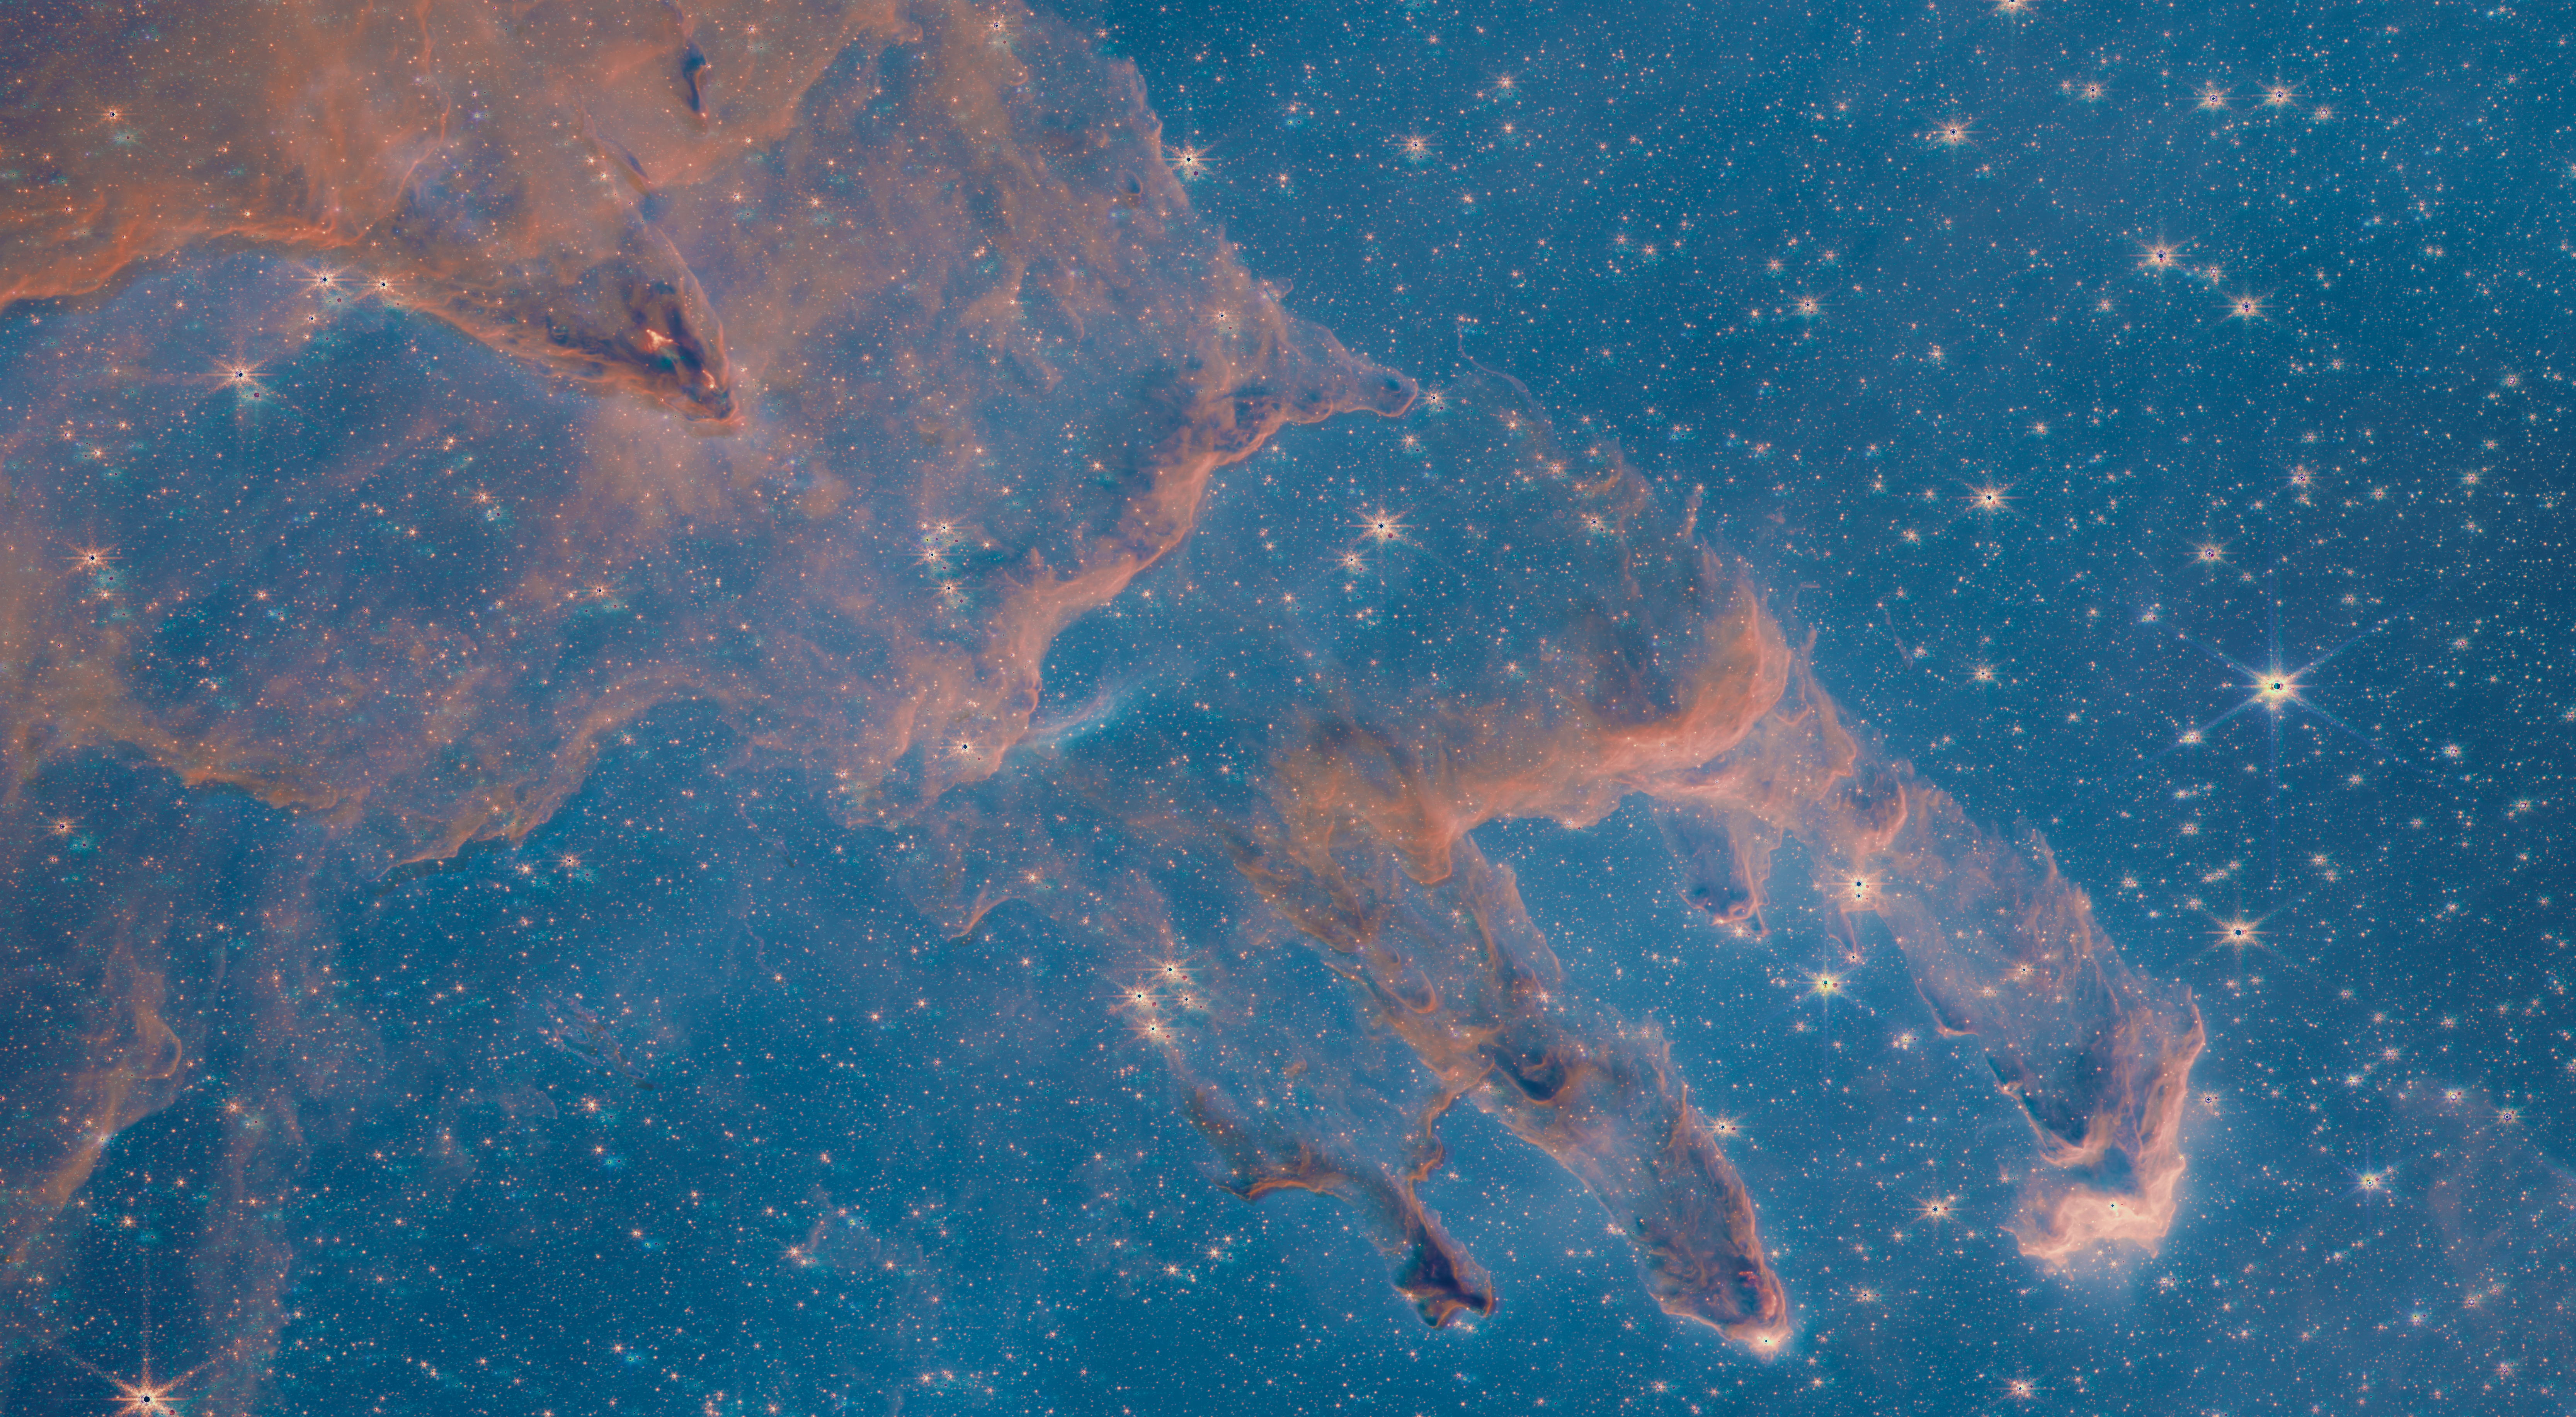
\includegraphics[width=0.75\textwidth]{./pillars/pillars.png}
	  \caption{Pillars of Creation Recreation}
	\end{figure}

	\begin{figure}[ht!]
	  \centering
	  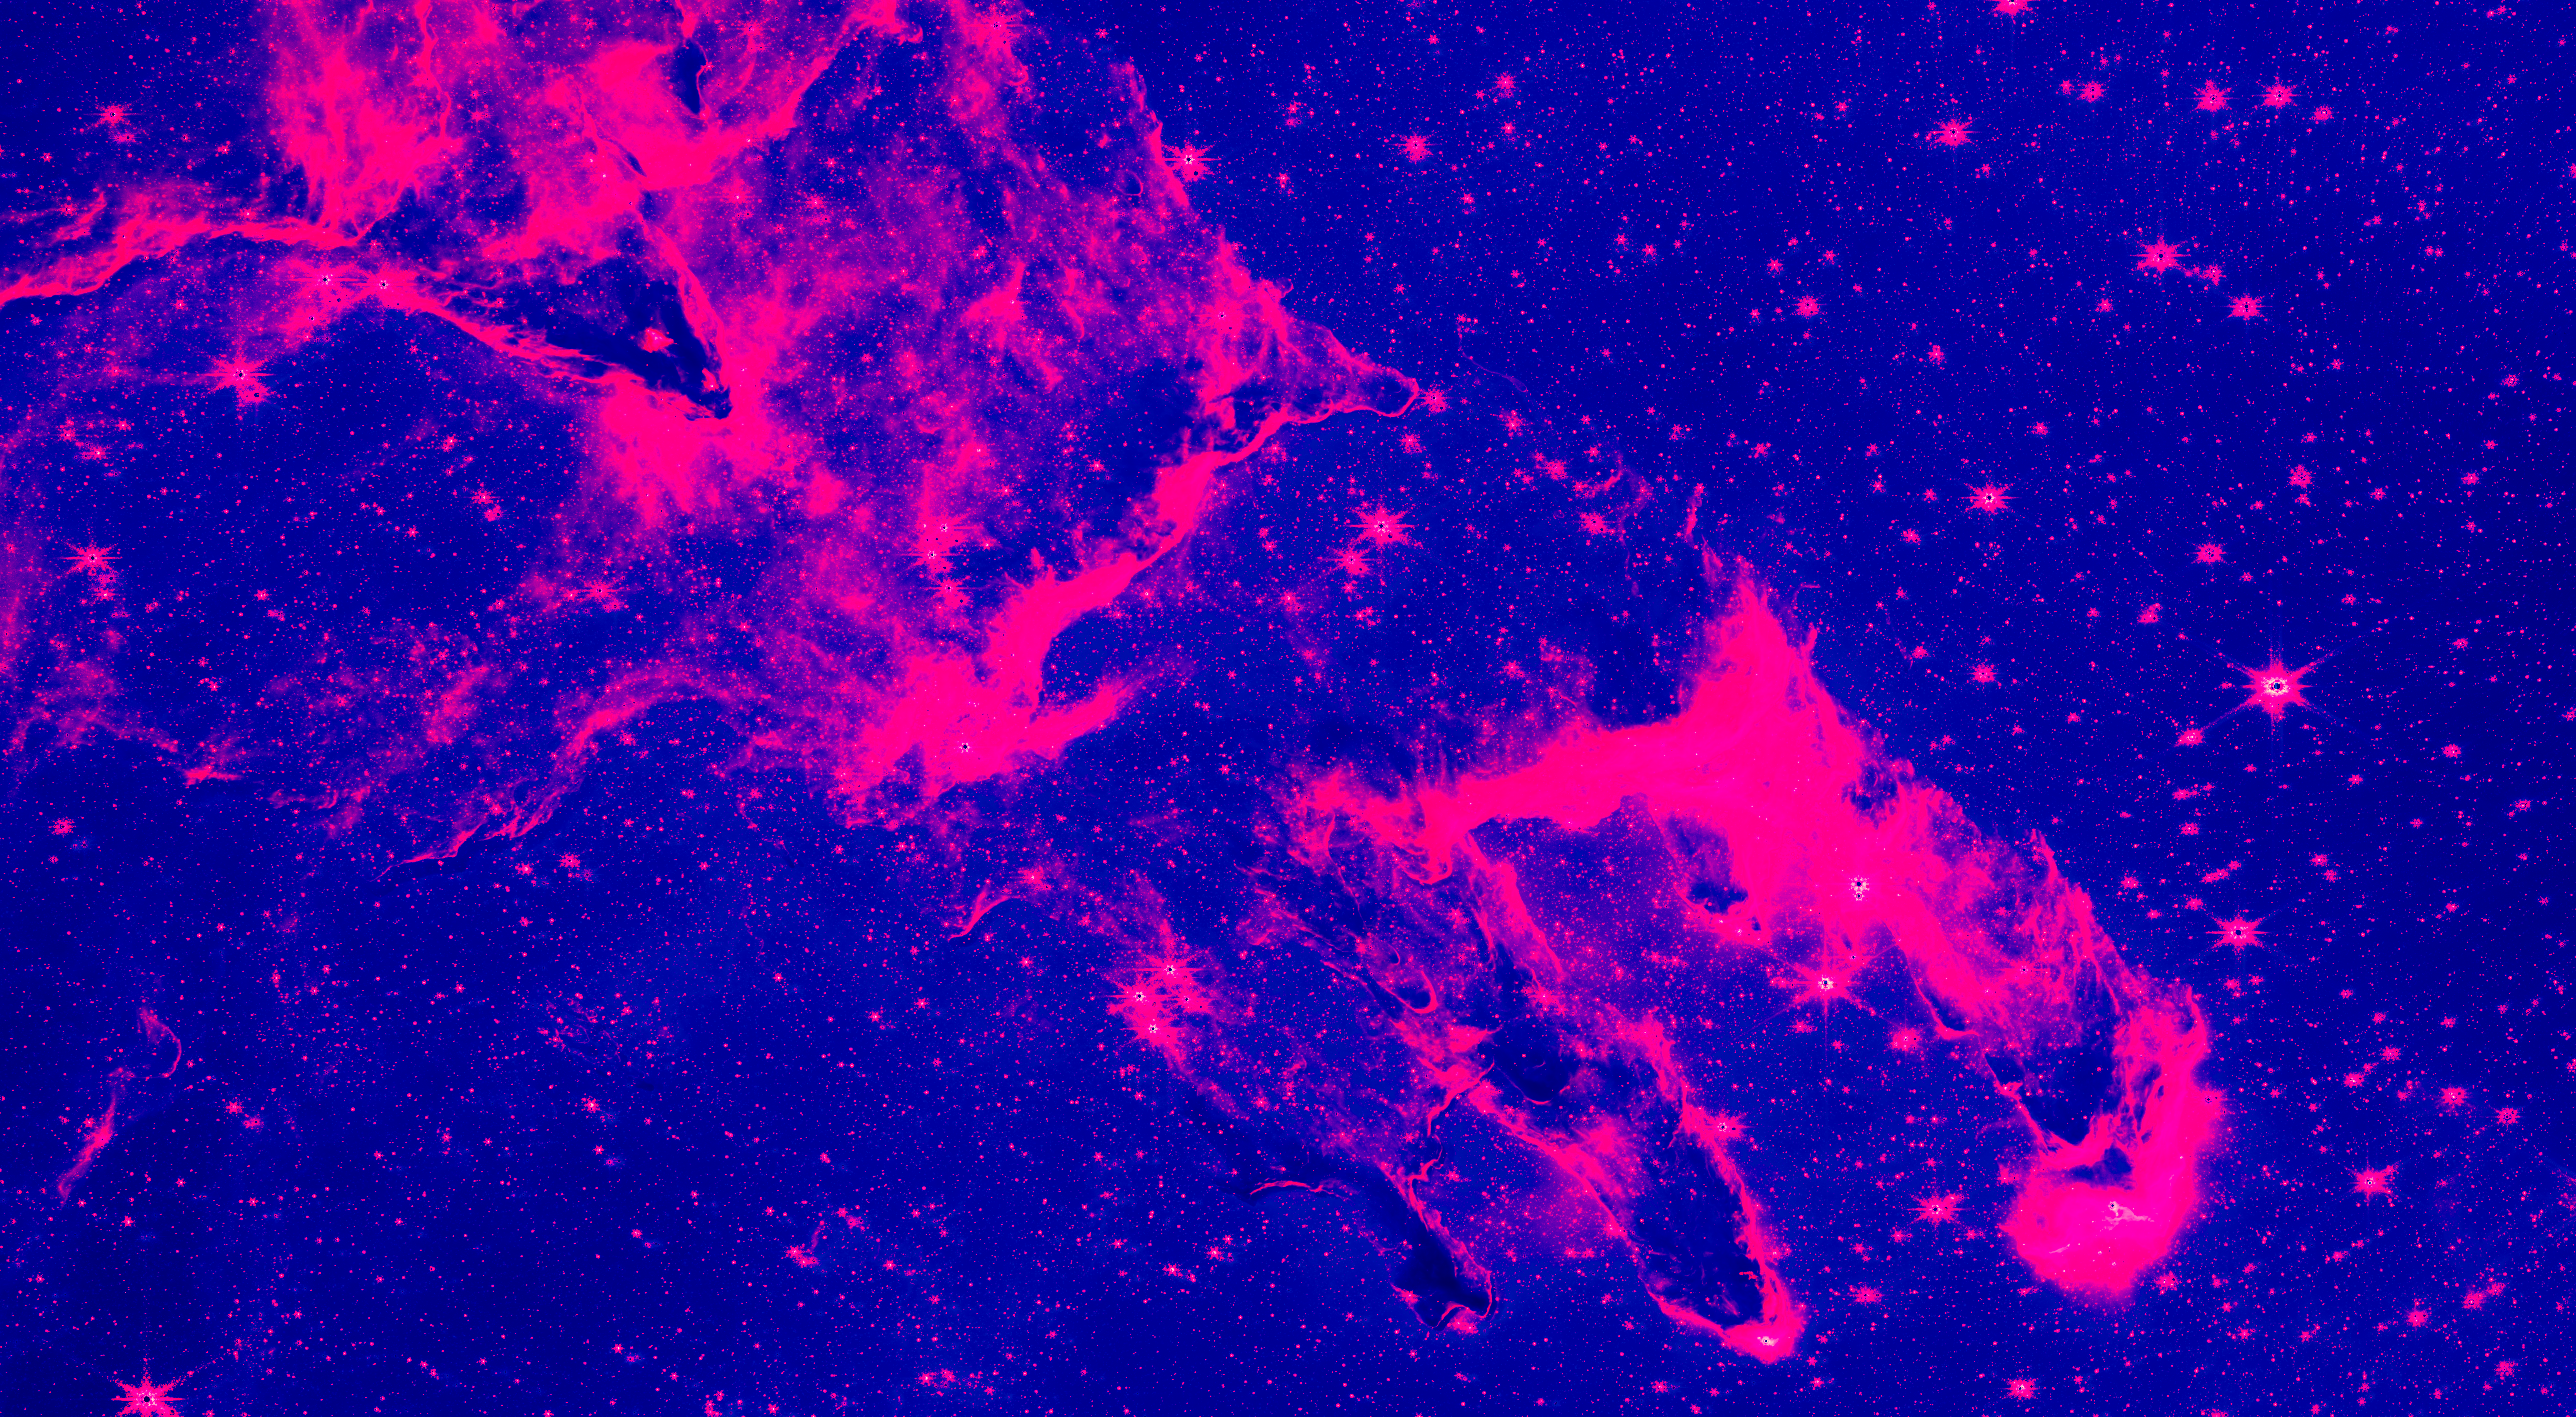
\includegraphics[width=0.75\textwidth]{./pillars/fun.png}
	  \caption{Pillars of Creation Fun Version}
	\end{figure}

\end{hwkProblem}

\end{document}
